\documentclass{article}

\usepackage{graphicx}
\usepackage{subfig}
\usepackage{tabularx}
\usepackage{lscape}
\begin{document}
%\begin{landscape}

\begin{figure}[h]
\vspace*{-2.75cm}
\advance\leftskip-3.0cm
\begin{tabularx}{\linewidth}{@{}XX@{}}
%
\begin{tabular}{ccc}
\multicolumn{2}{c}{\textbf{Wild type Drosophila (Hexamer Test) - motif pair correlations at 50bp apart}} \\

\subfloat[Motif GC content of 0\%]{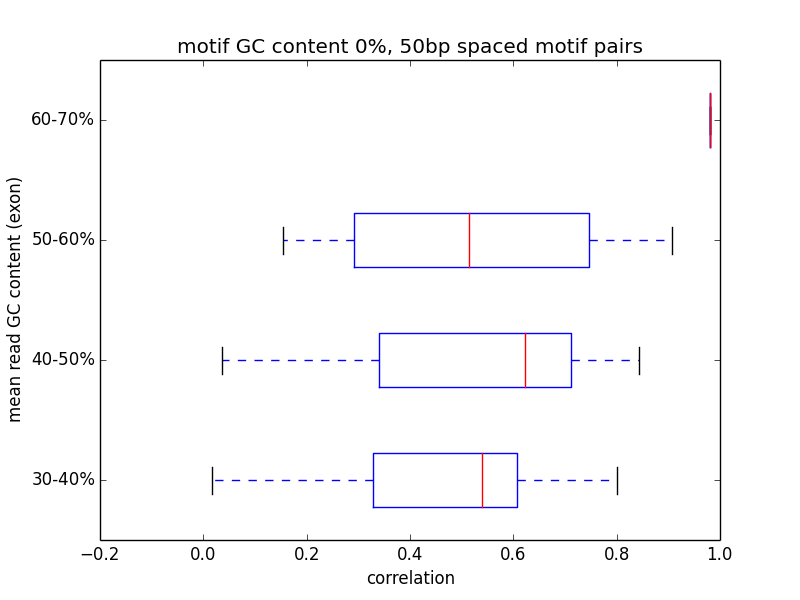
\includegraphics[scale=0.45]{./box-motif-gc-0pc-50bp-spaced.png}} 
   & \subfloat[Motif GC content of 25\%]{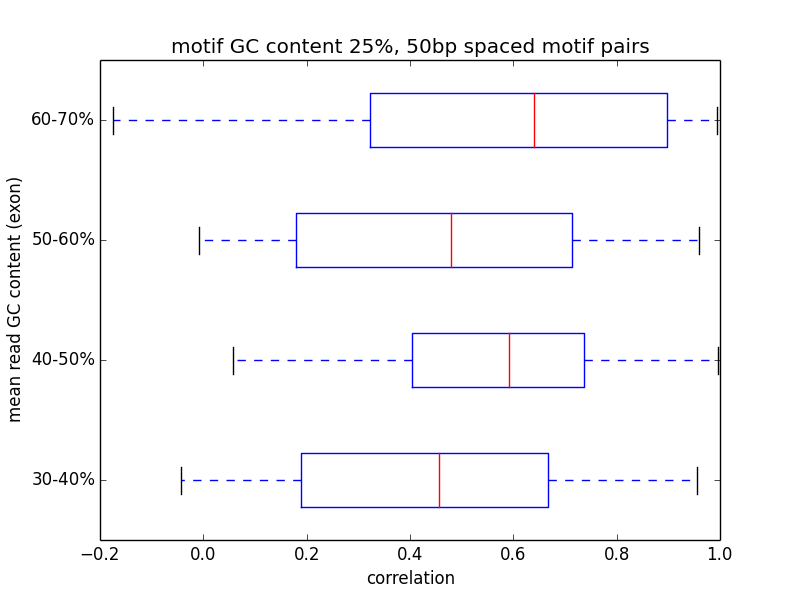
\includegraphics[scale=0.45]{./box-motif-gc-25pc-50bp-spaced.png}} \\
   
\multicolumn{2}{c}{\subfloat[Motif GC content of 50\%]{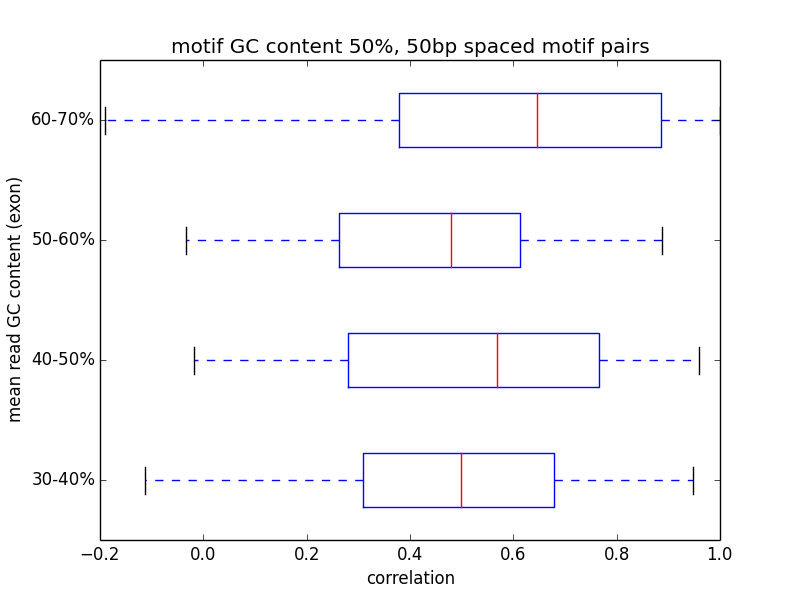
\includegraphics[scale=0.45]{./box-motif-gc-50pc-50bp-spaced.png}}} \\    
  
\subfloat[Motif GC content of 75\%]{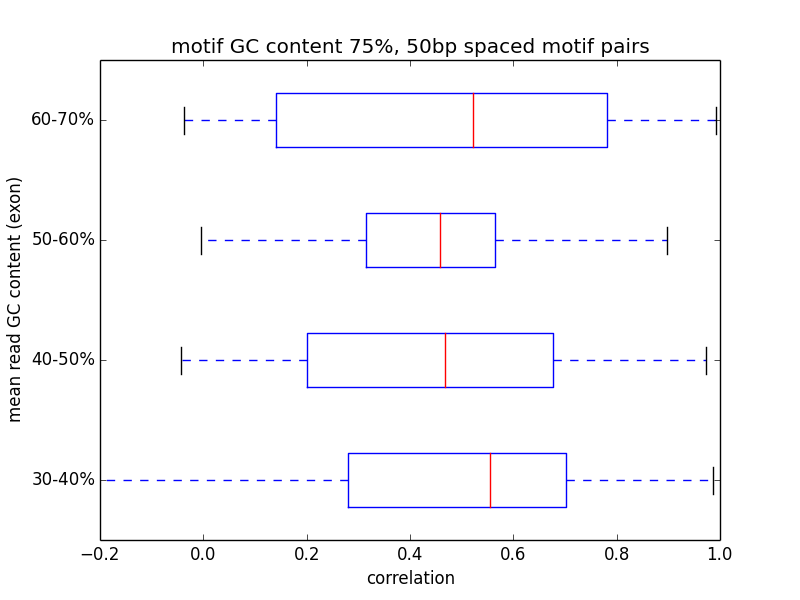
\includegraphics[scale=0.45]{./box-motif-gc-75pc-50bp-spaced.png}} 
   & \subfloat[Motif GC content of 100\%]{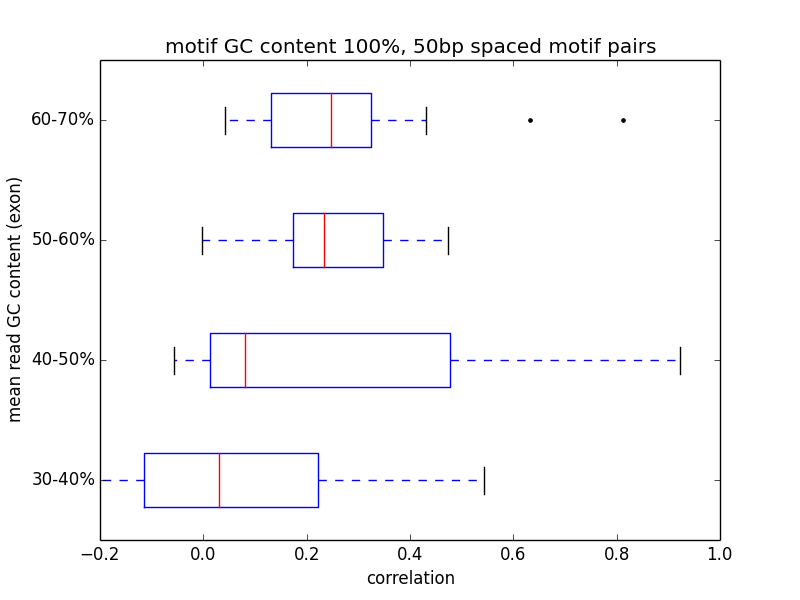
\includegraphics[scale=0.45]{./box-motif-gc-100pc-50bp-spaced.png}} 
\end{tabular}

\end{tabularx}

\caption{Box and whisker plots of motif pair correlations at a distance of 50bp apart with varying median GC content and varying motif GC content.}\label{foo}
\end{figure}

%\end{landscape}


\end{document}




%\centering
%\includegraphics[scale=0.40]{./box-motif-gc-0pc-10bp spaced.png}
%\caption[10 spaced]{\label{fig:10}Description/explanation of method} 
%\end{figure}
